\subsection{Results}
\subsubsection{Cropping}
Cropping refers to 27 regions that defined by two planes along each coordinate axis of the volume and can be independently turned on (visible) or off (invisible) to produce a variety of different cropping effects, as shown in Figure~\ref{fig:cropping}. Cropping is implemented by determining the cropping region of each sample location along the ray and including only those samples that fall within a visible region.

\begin{figure}
\centering
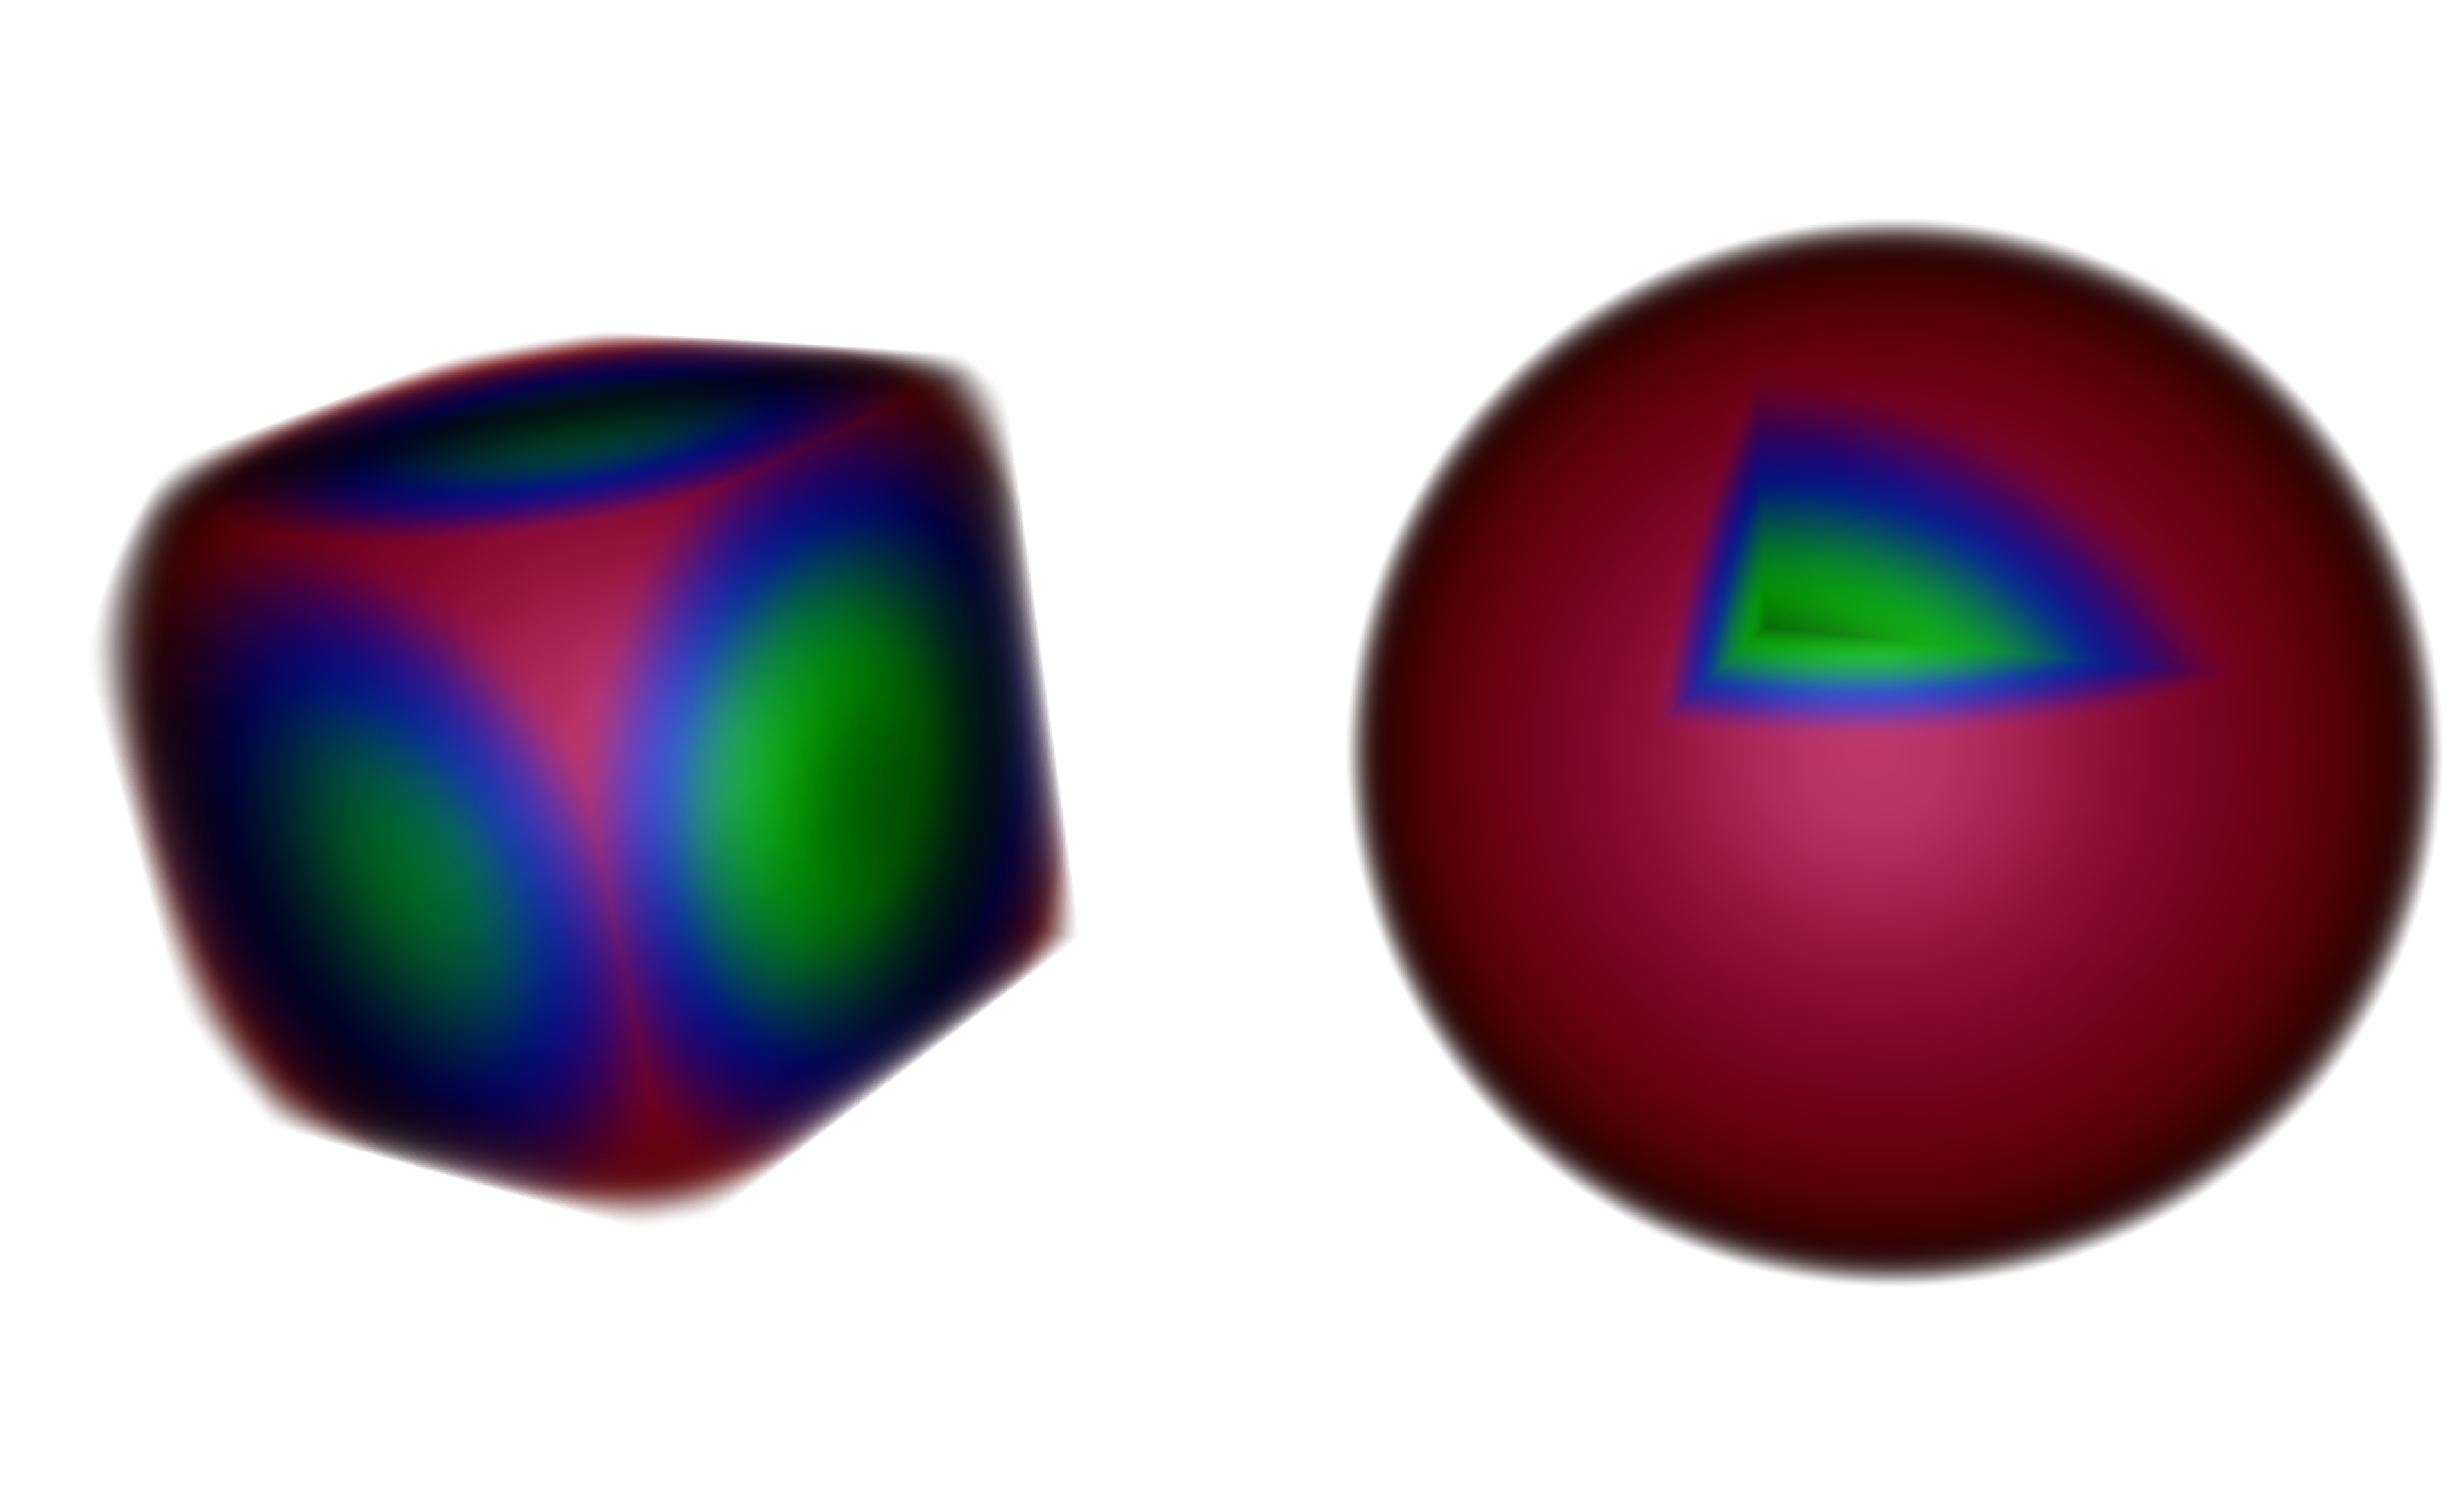
\includegraphics[width=2.5in]{SphereCropping.png}
\caption{Figure 3. A sphere is cropped using two different configurations of cropping regions.}
\label{fig:cropping}
\end{figure}

\subsubsection{Wide Support of Data Types} 
The vtkGPURayCastMapper supports most data types such as short, int, float, and double and both point and cell data types. Bias are scale are computed and applied to the scalars in the fragment shader to normalize the scalars between 0-1 range. 

\subsubsection{Clipping}
A set of infinite clipping planes can be defined to clip the volume to reveal inner detail, as shown in Figure 4.  Clipping is implemented by determining the visibility of each sample along the ray according to whether that location is excluded by the clipping planes.A set of infinite clipping planes can be defined to clip the volume to reveal inner detail, as shown in Figure 4.  Clipping is implemented by determining the visibility of each sample along the ray according to whether that location is excluded by the clipping planes.

\begin{figure}
\centering
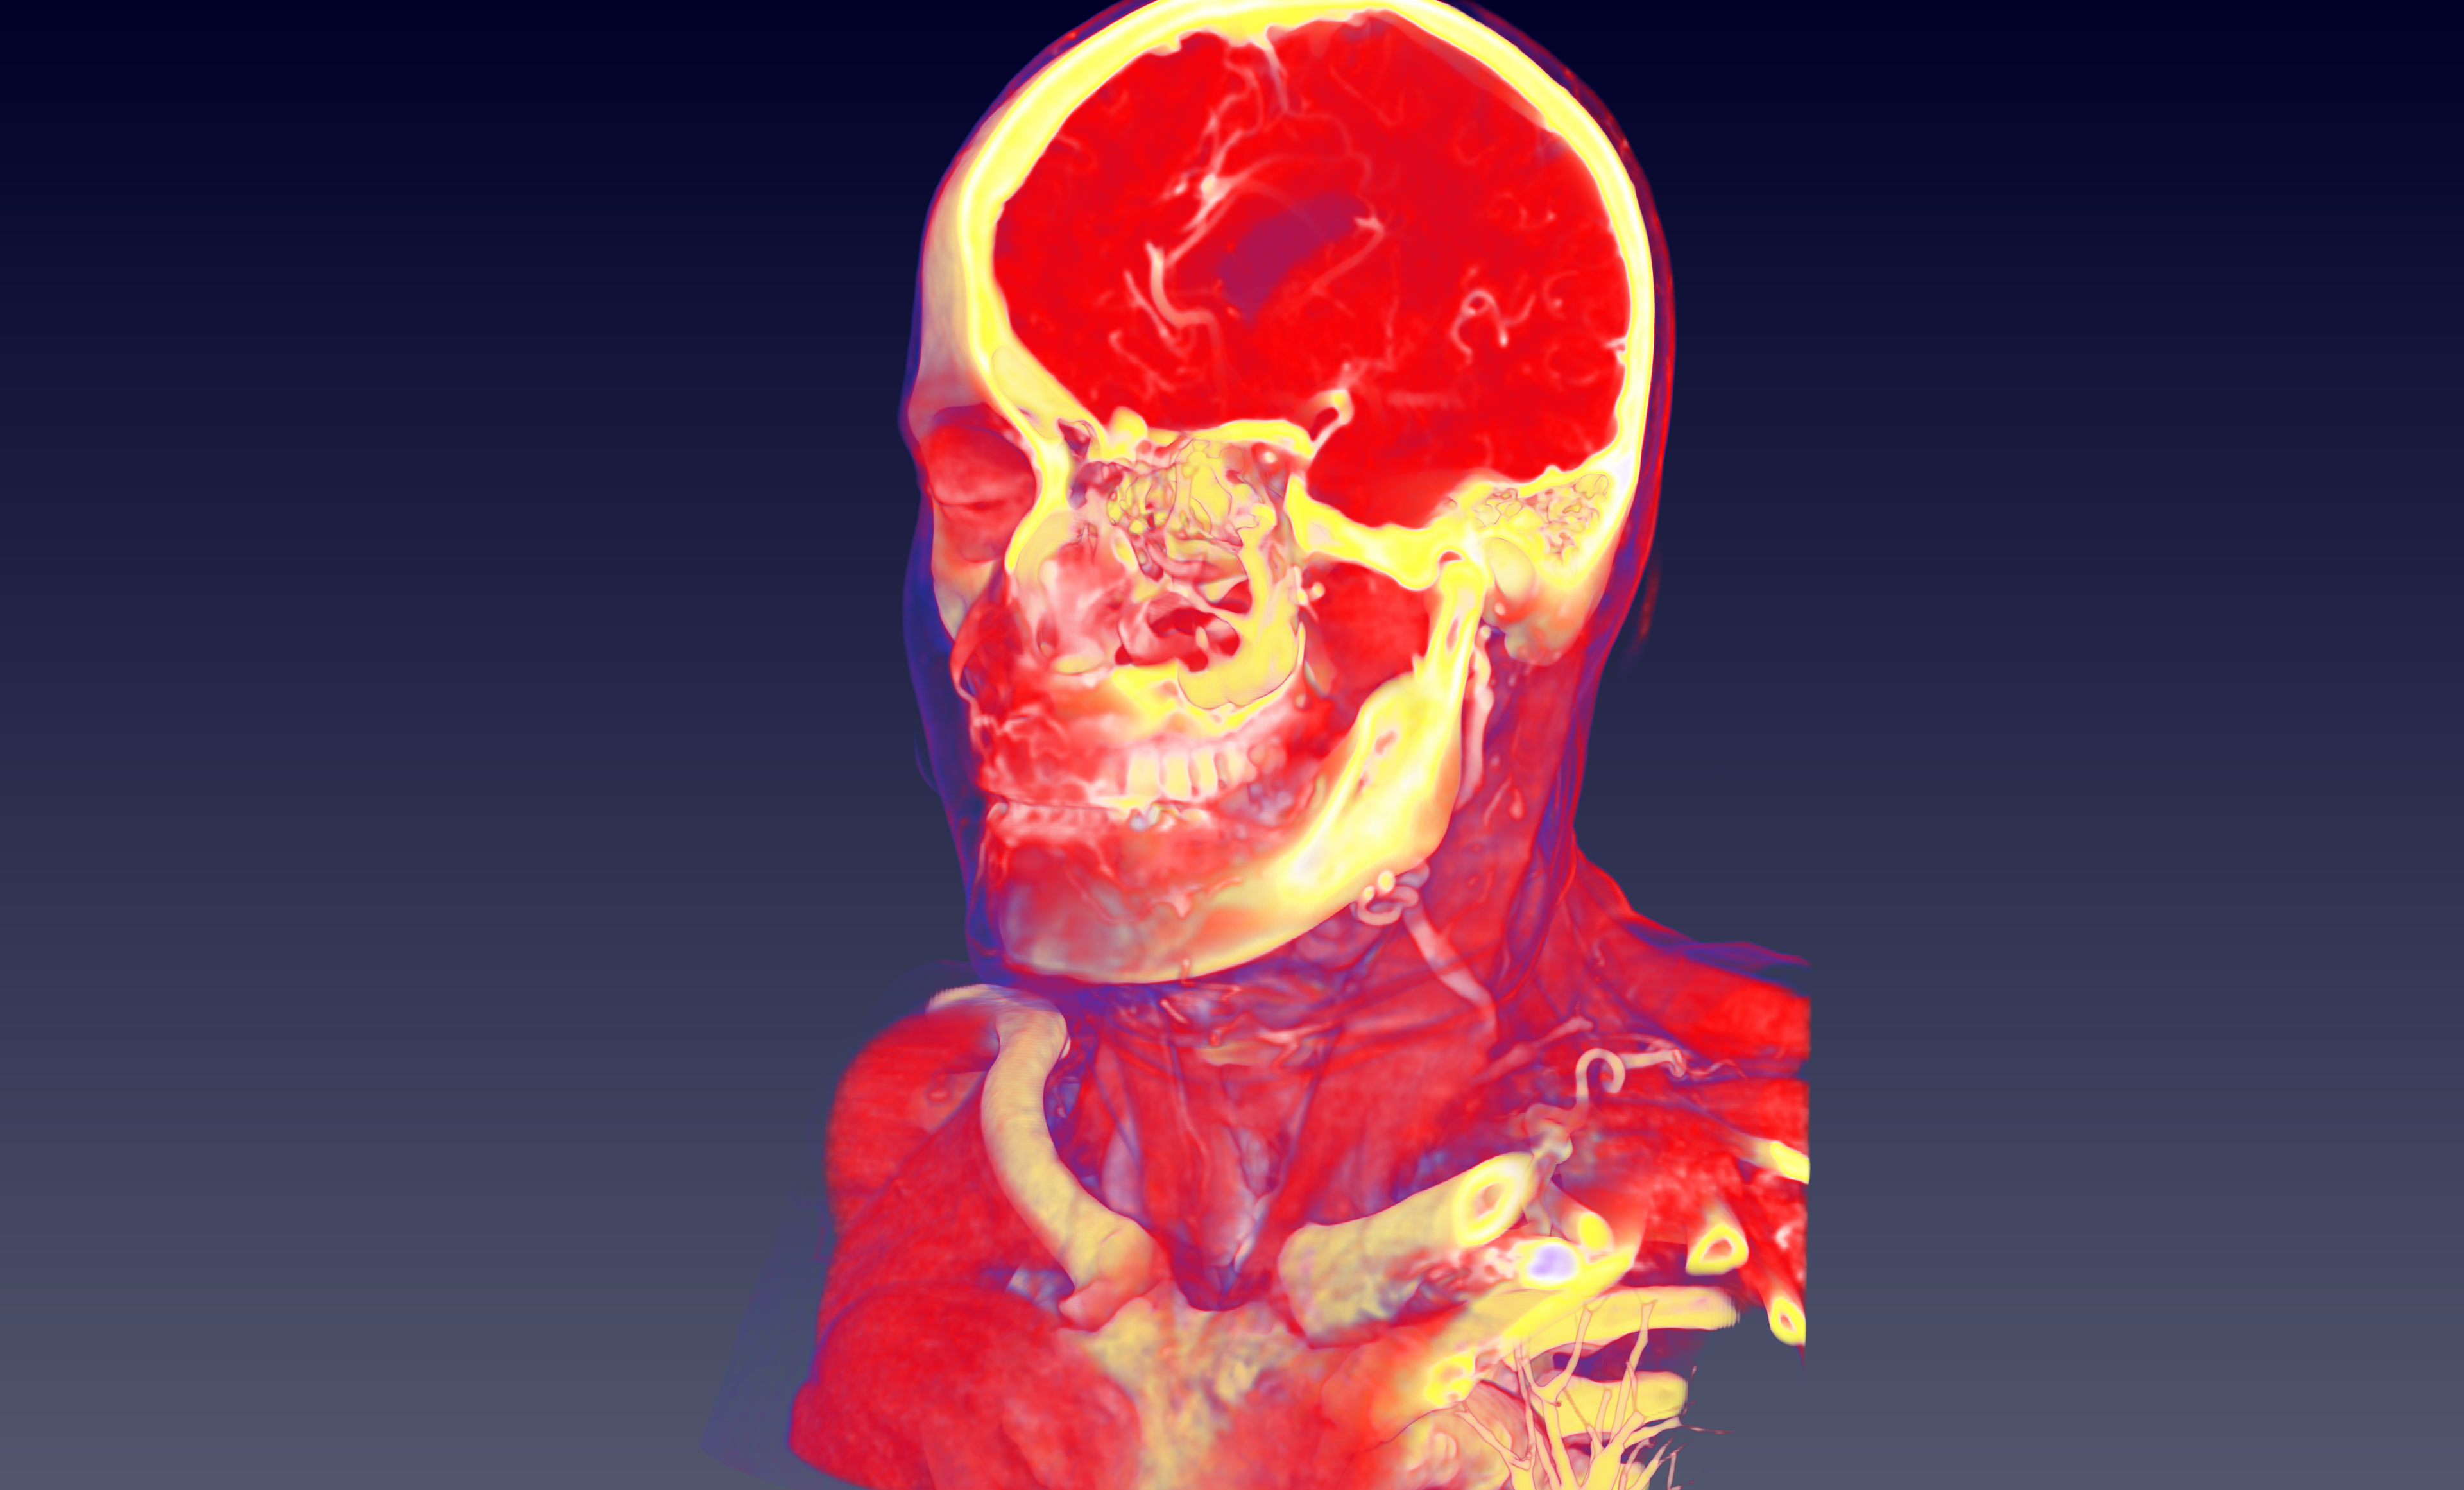
\includegraphics[width=2.5in]{HeadClippingOblique.png}
\caption{Figure 4. Top: An example of an oblique clipping plane. Bottom: A pair of parallel clipping planes clip the volume, rendered without (left) and with (right) shading.}
\label{fig:clipping}
\end{figure}

\subsubsection{Blending Modes}
The mapper supports composite blending, minimum intensity projection, maximum intensity projection, and additive blending. Each of these blending modes are useful for a particular use-case in medical computing. The most common one which is also the default is the composite blending mode. See Figure~\ref{fig:blendingmodes} for an example of composite blending, maximum intensity projection, and additive blending on the same data.

\begin{figure*}
\centering
\begin{subfigure}{.6\columnwidth}
    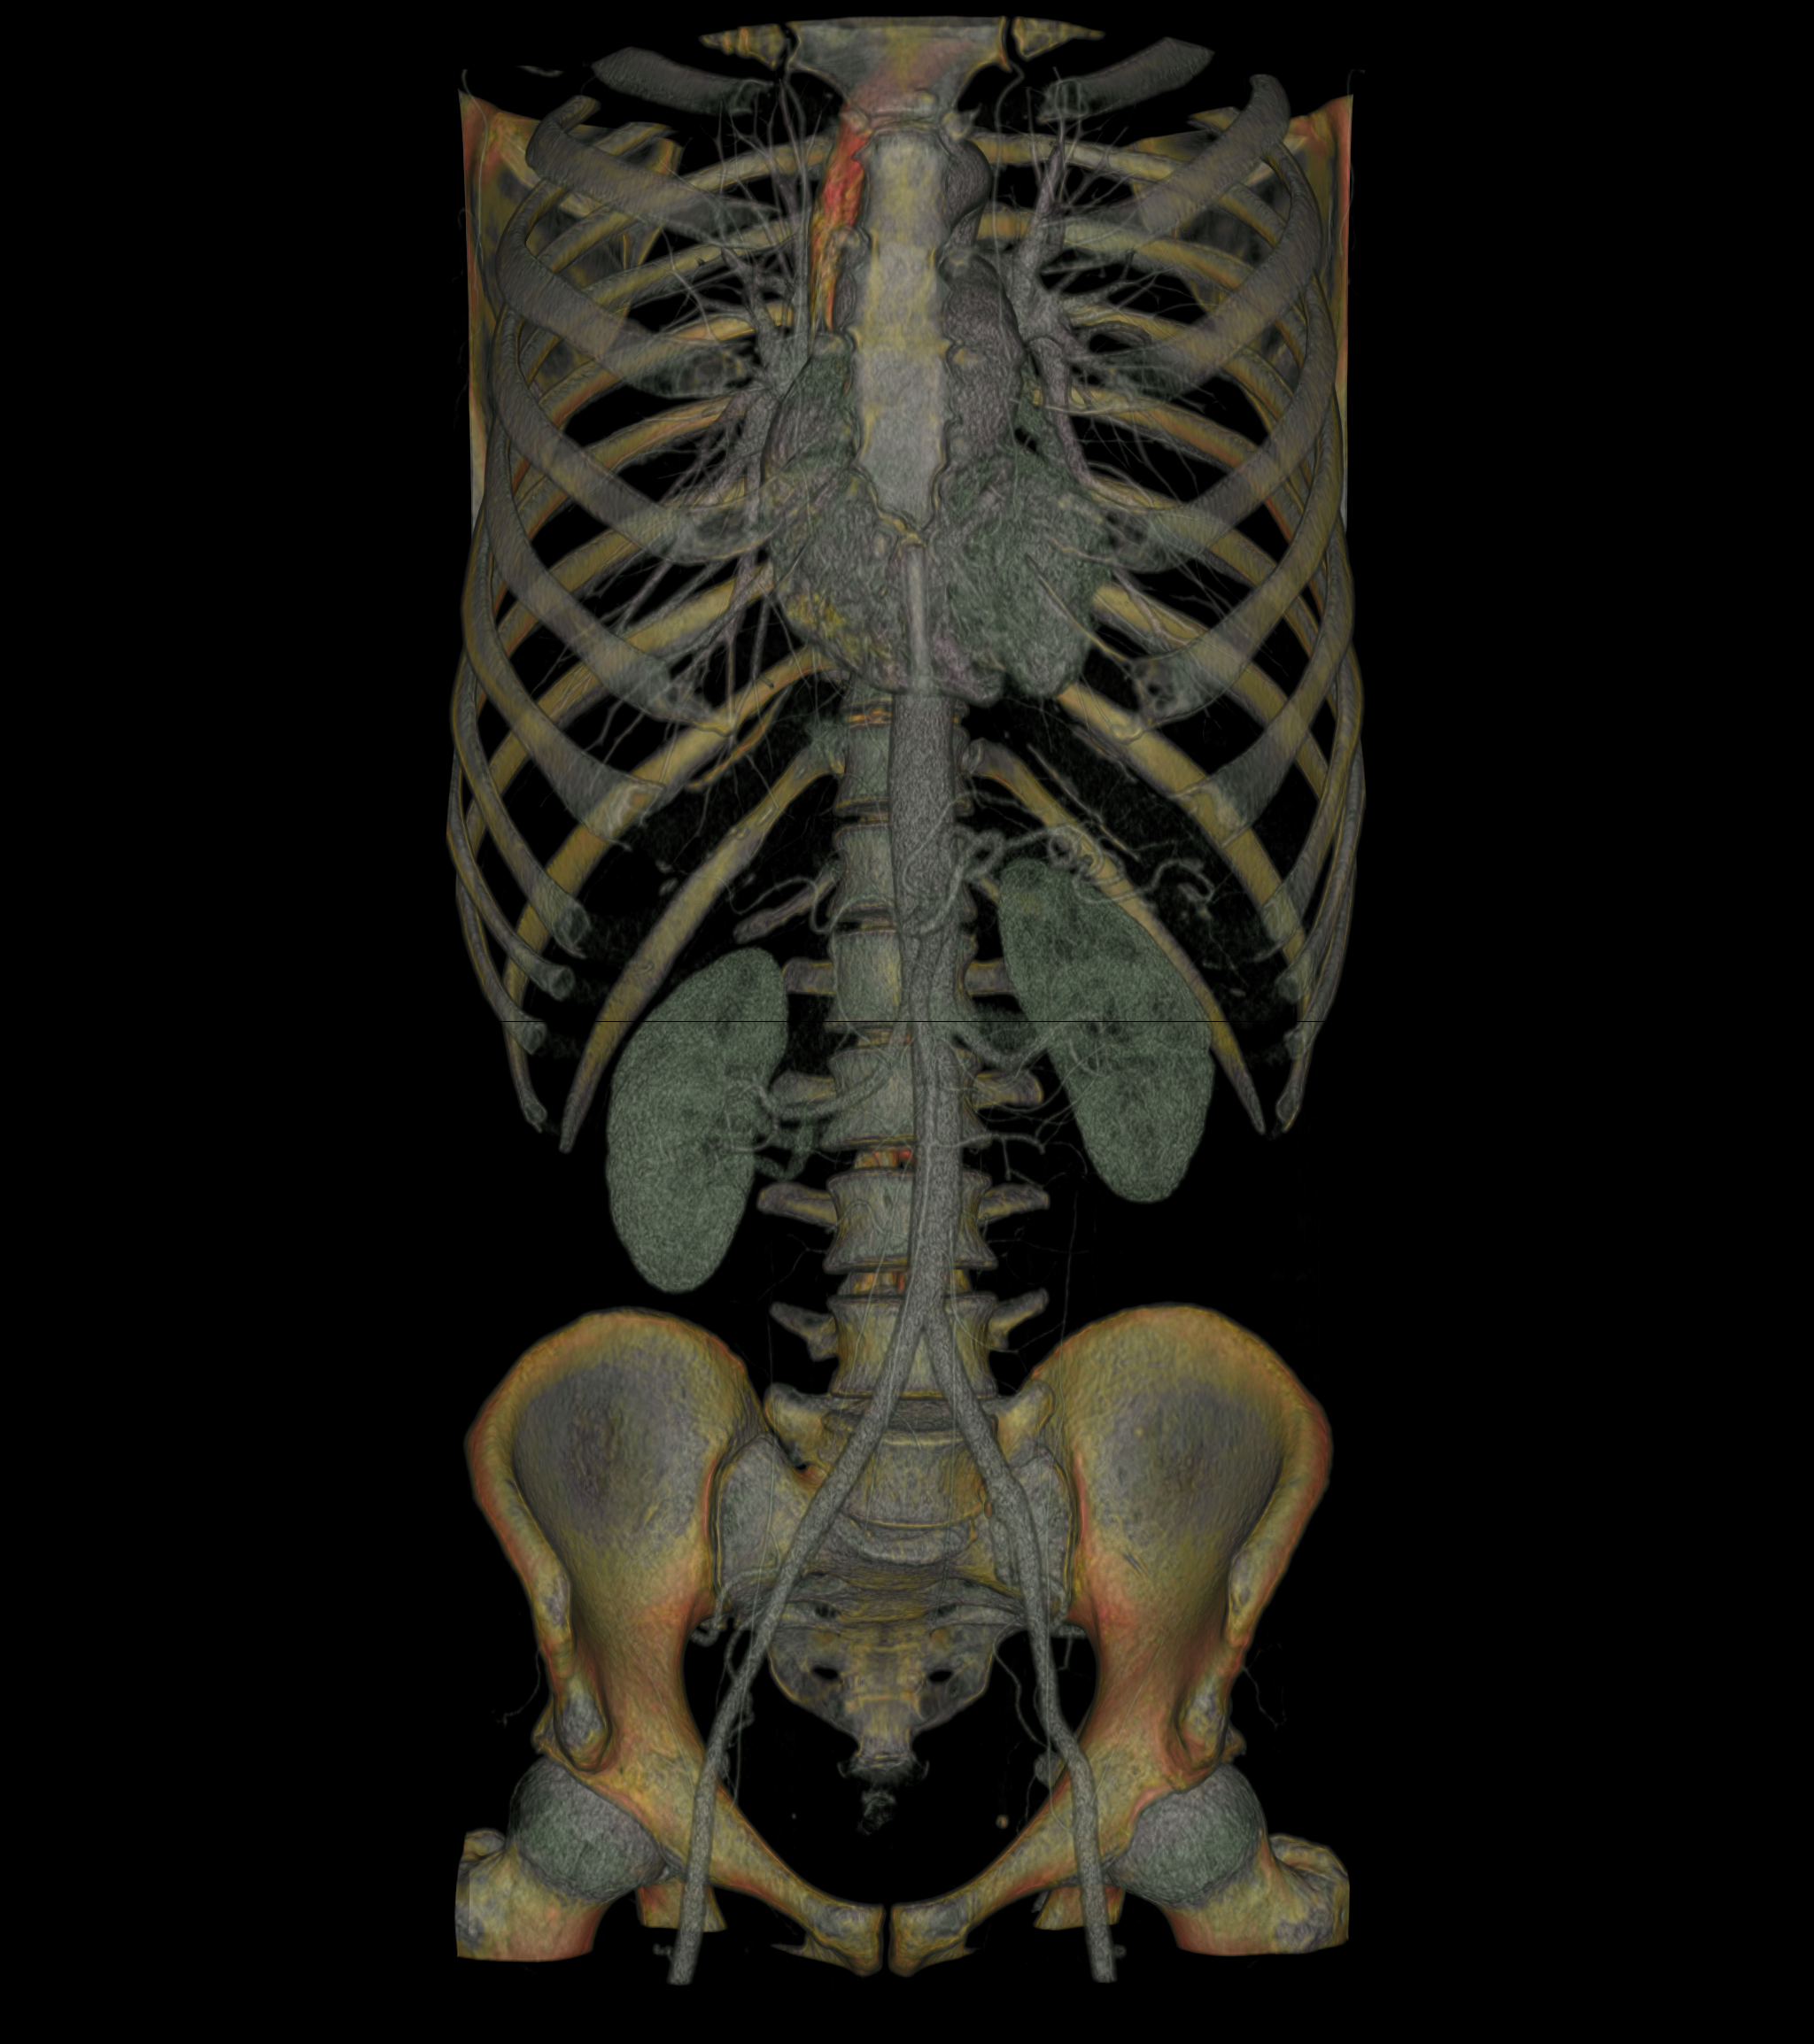
\includegraphics[width=\columnwidth]{TorsoBlendingComposite.png}
\end{subfigure}
\begin{subfigure}{.6\columnwidth}   
    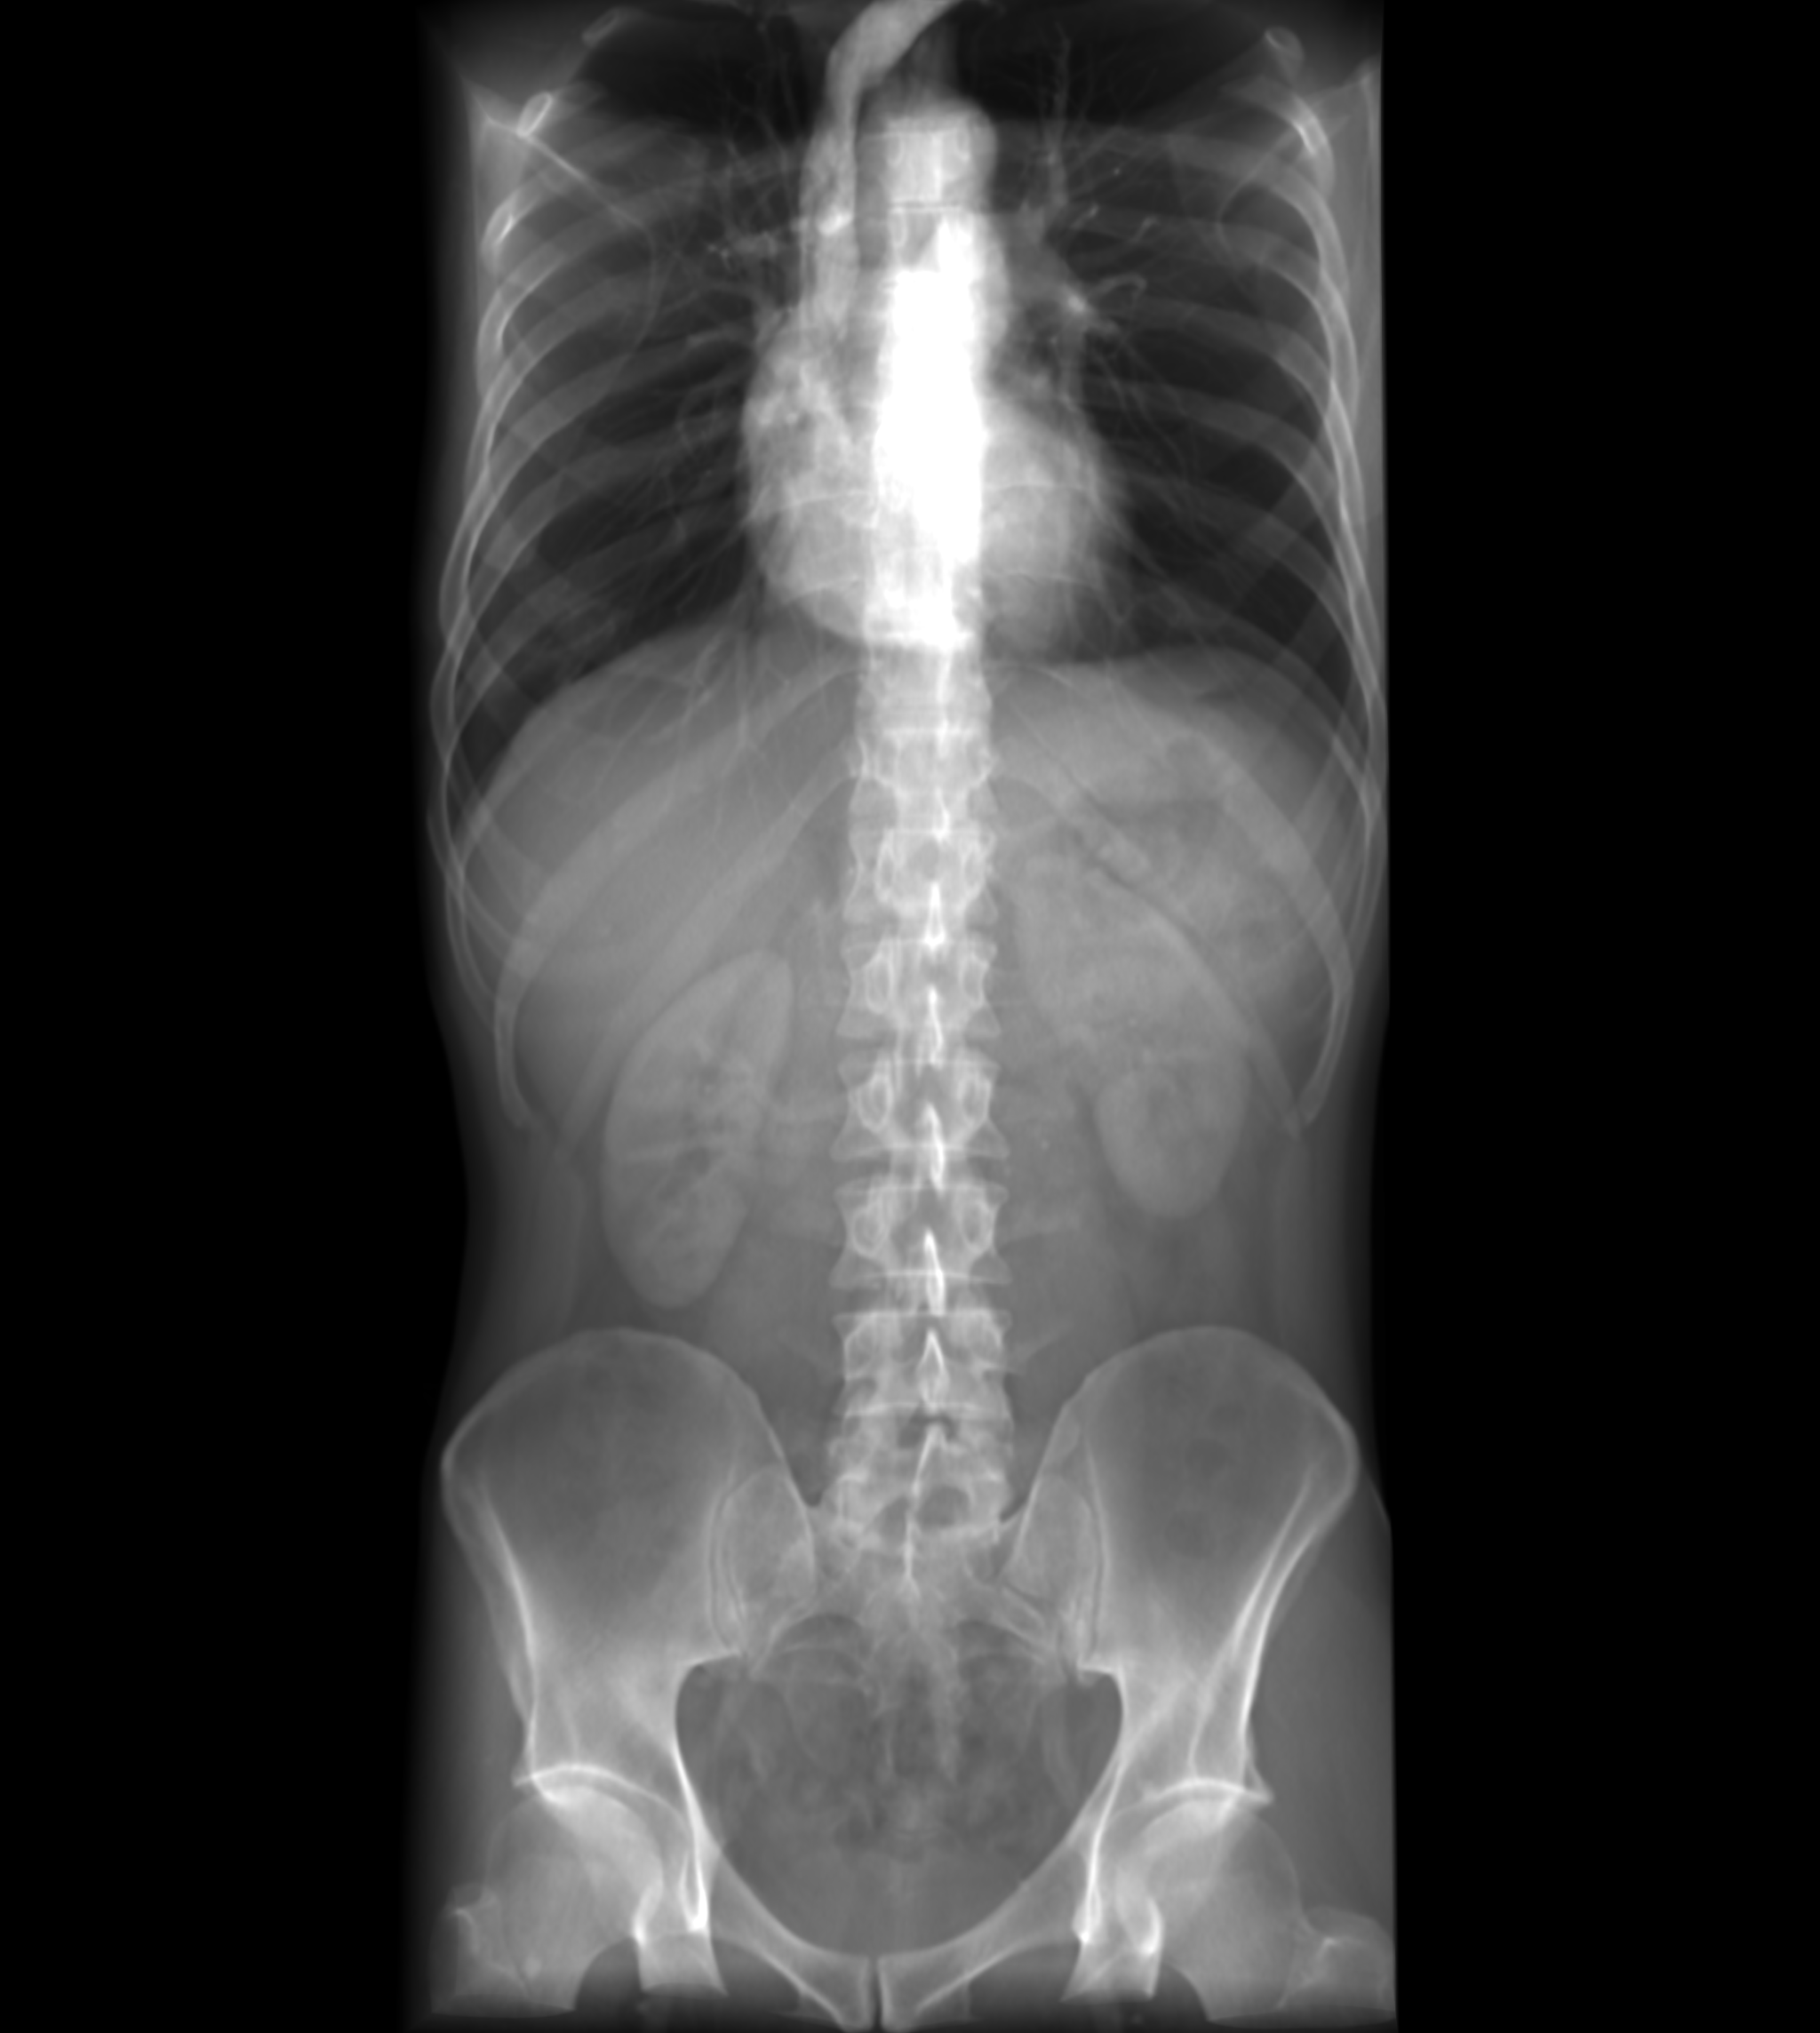
\includegraphics[width=\columnwidth]{TorsoBlendingAdditive.png}
\end{subfigure} 
\begin{subfigure}{.6\columnwidth}
    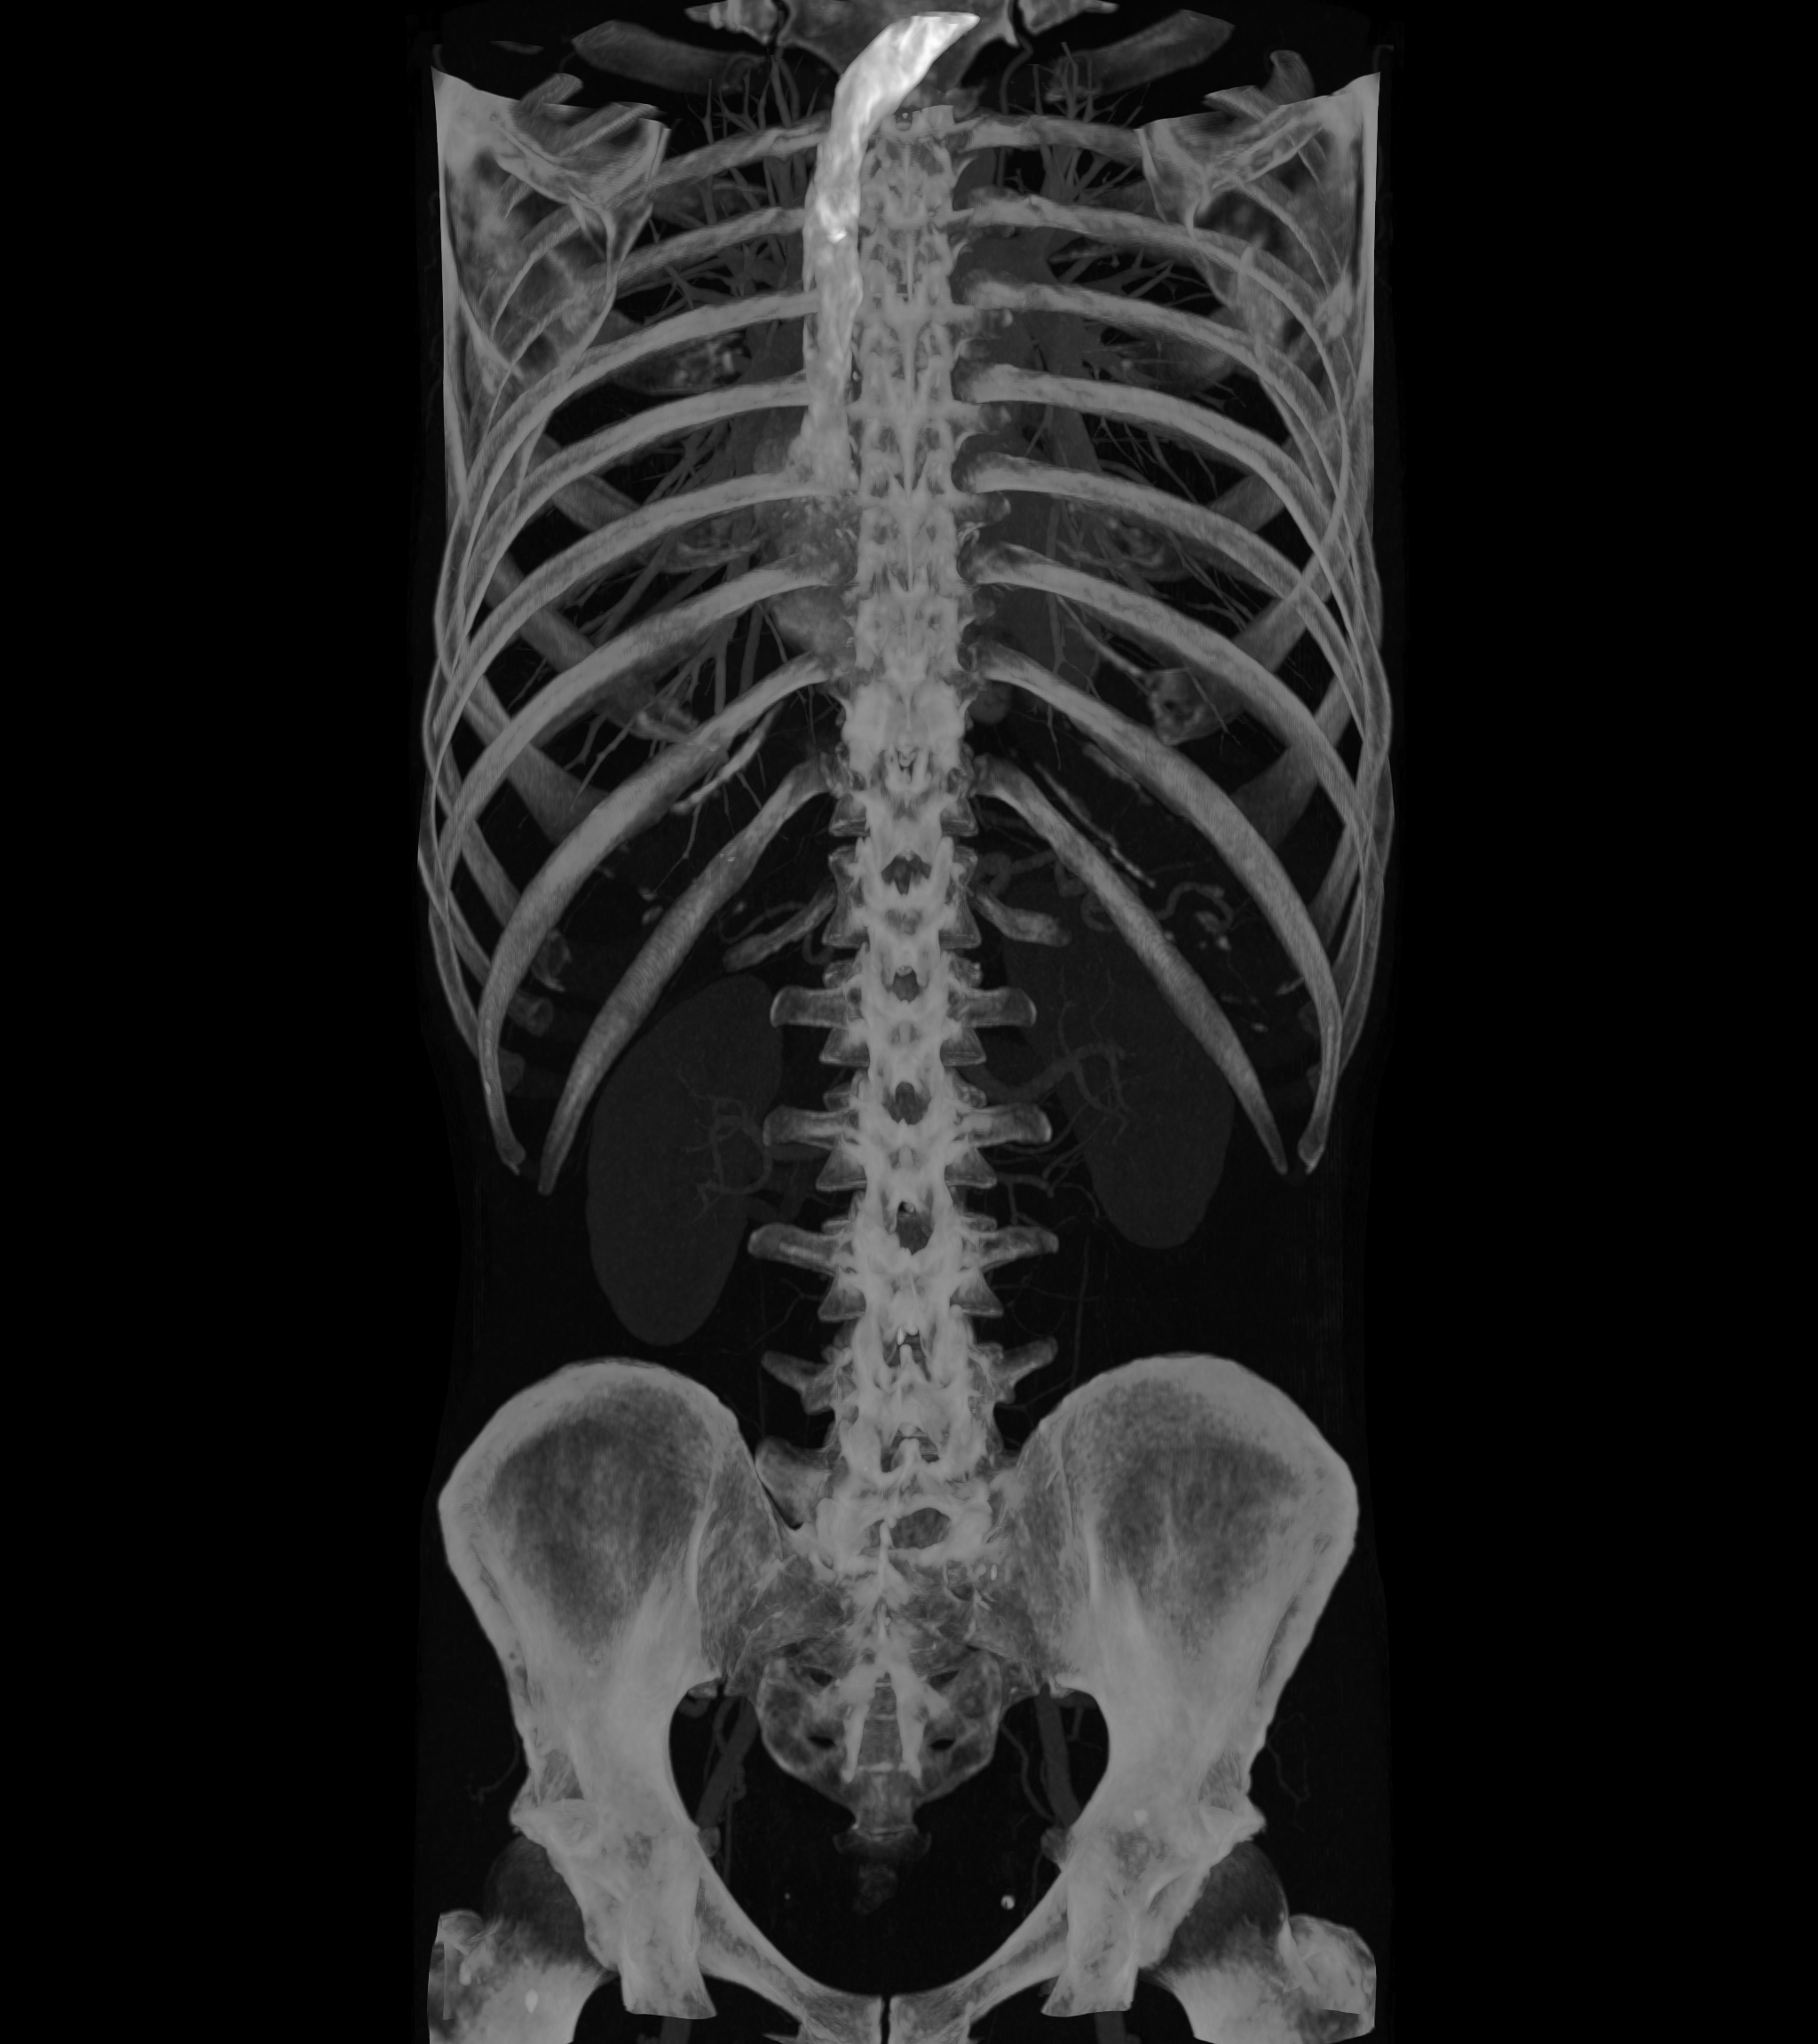
\includegraphics[width=\columnwidth]{TorsoBlendingMIP.png}
\end{subfigure}
\caption{Rendering with and without gradient opacity transfer function.}
\label{fig:blendingmodes}
\end{figure*}

\subsubsection{Masking}
Both binary and label masks are supported. With binary masks, the value in the masking volume indicates visibility of the voxel in the data volume. When a label map is in use, the value in the label map is used to select different rendering parameters for that sample.  See Figure 5 for an example of label data masks.

\subsubsection{Opacity Modulated by Gradient Magnitude}
A transfer function mapping the magnitude of the gradient to an opacity modulation value can be used to essentially perform edge detection (de-emphasize homogenous regions) during rendering. See ~\ref{fig:gradient} for an example of rendering with and without the use of a gradient opacity transfer function.

\begin{figure*}
\centering
   \begin{subfigure}[b]{0.5\textwidth}
   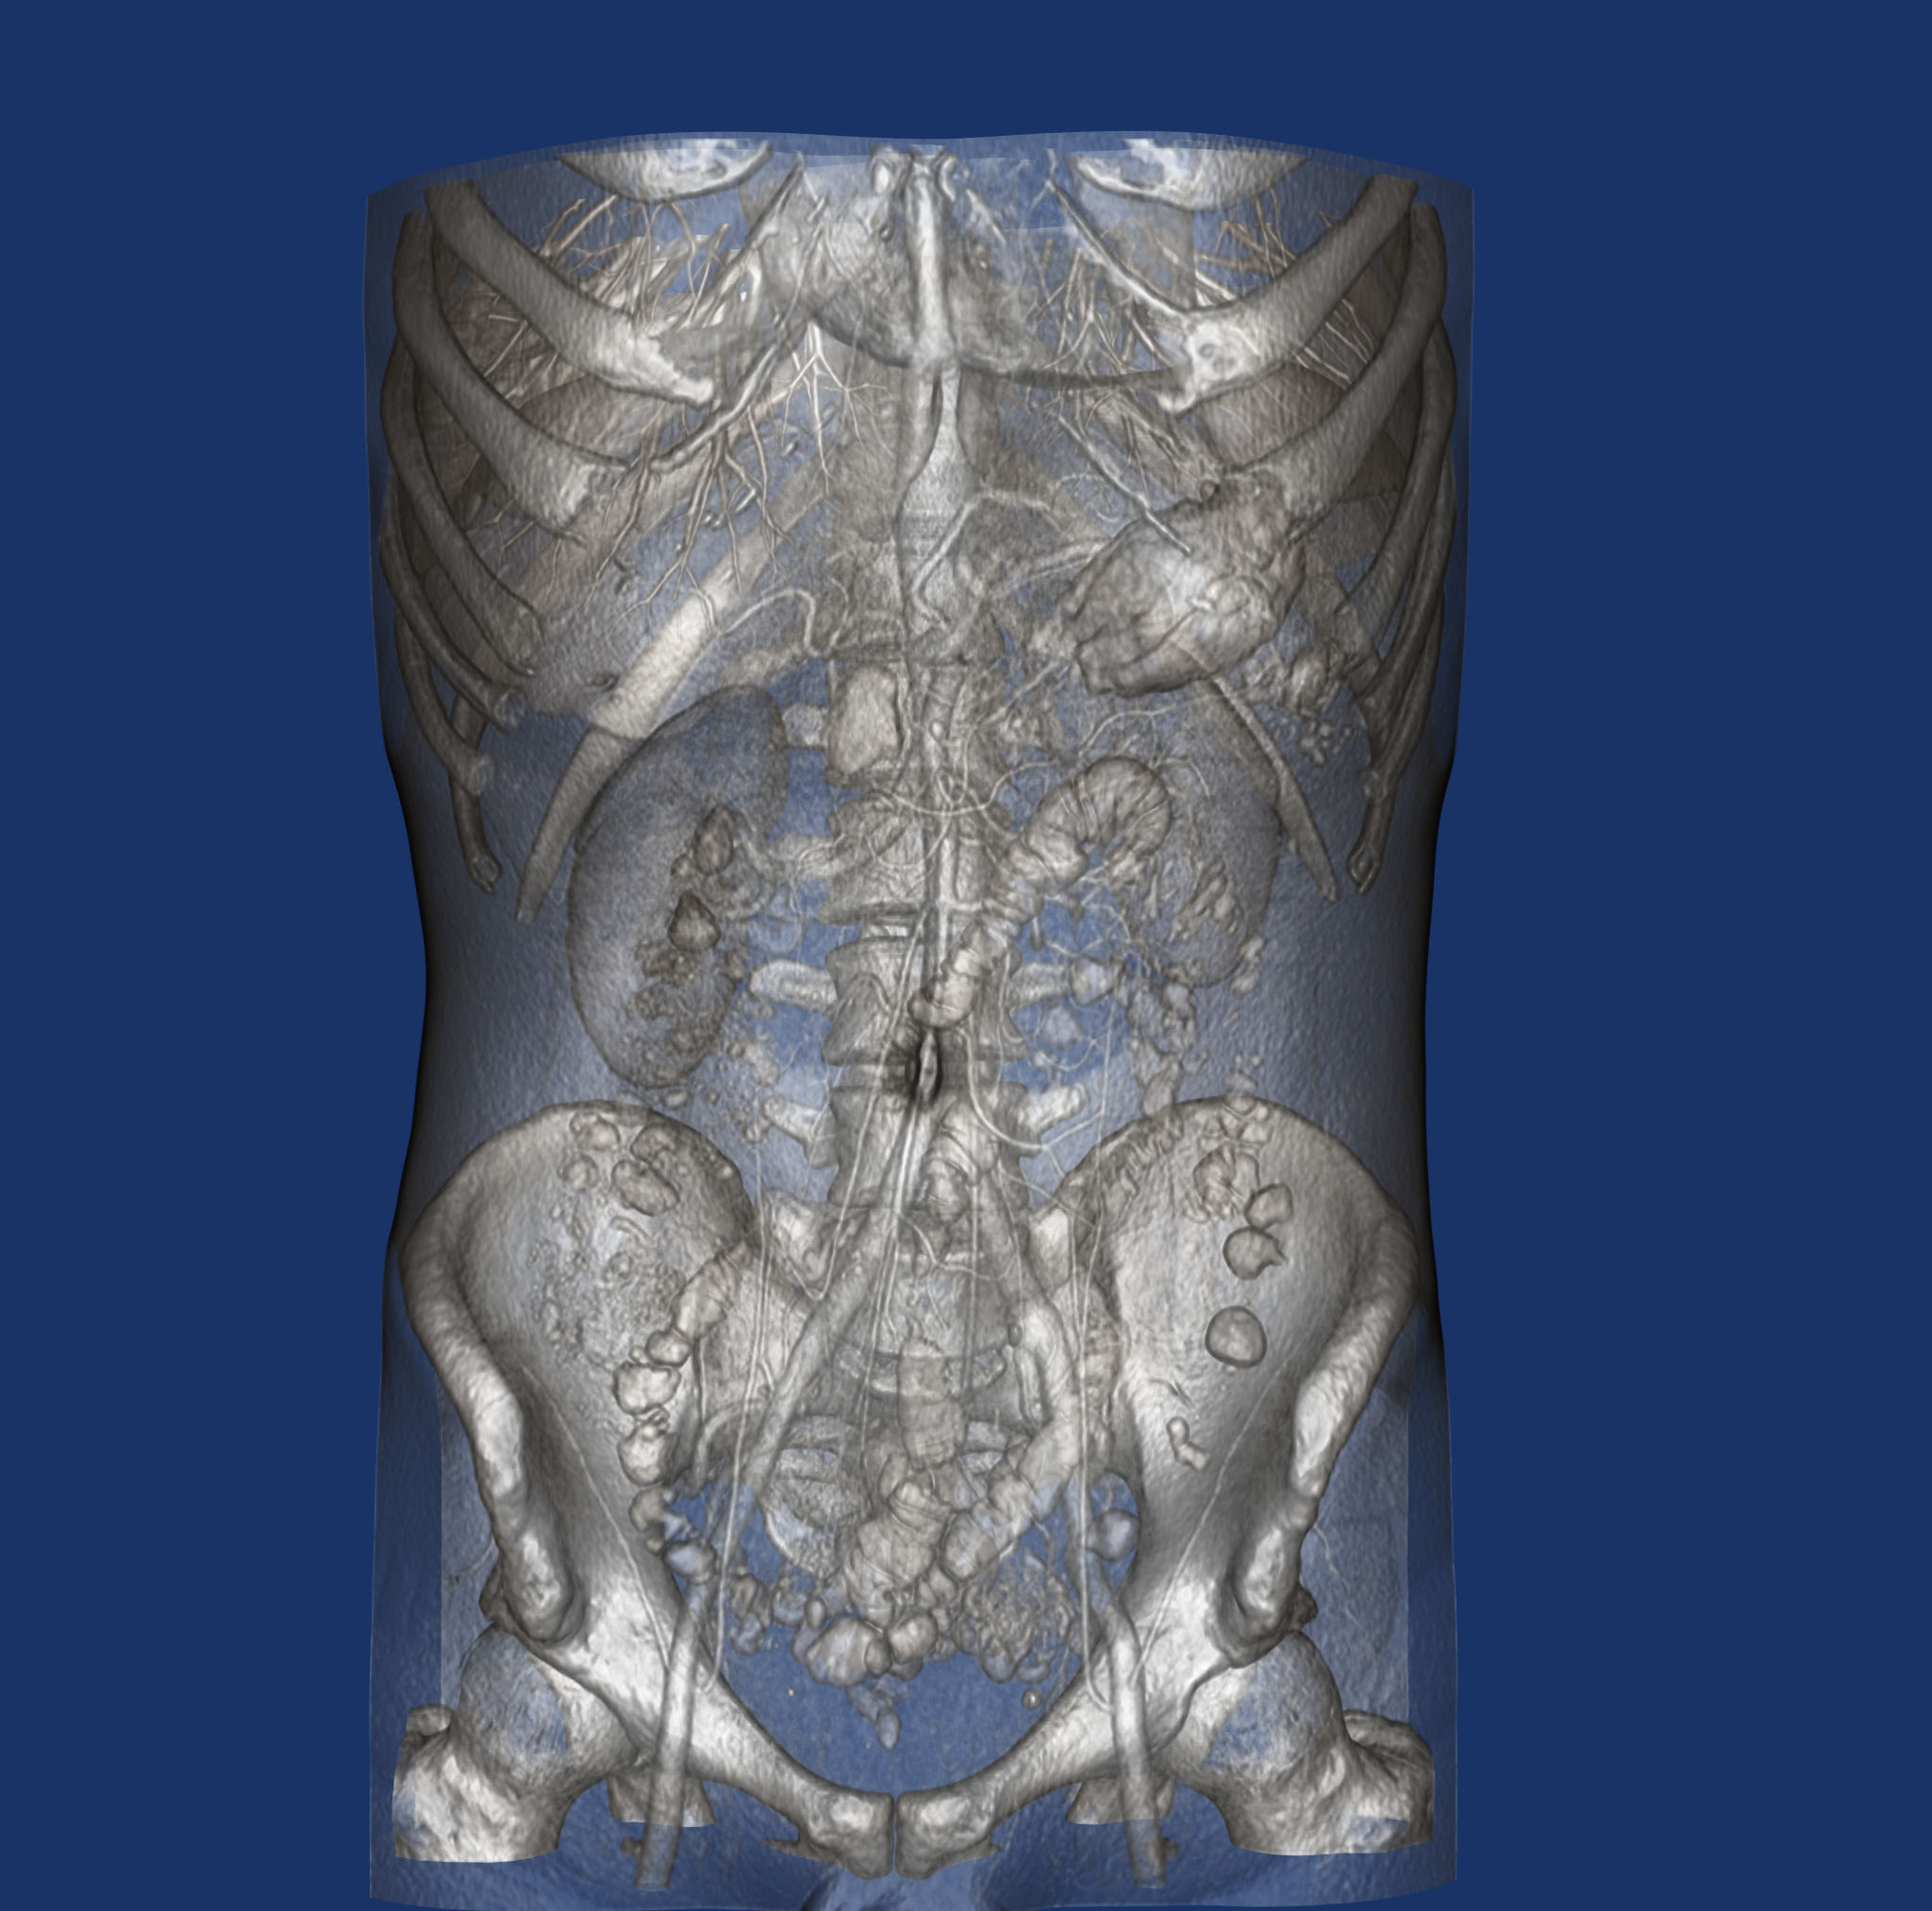
\includegraphics[width=1\linewidth]{TorsoGradient.png}
   \caption{}
   \label{fig:Ng1} 
\end{subfigure}

\begin{subfigure}[b]{0.5\textwidth}
   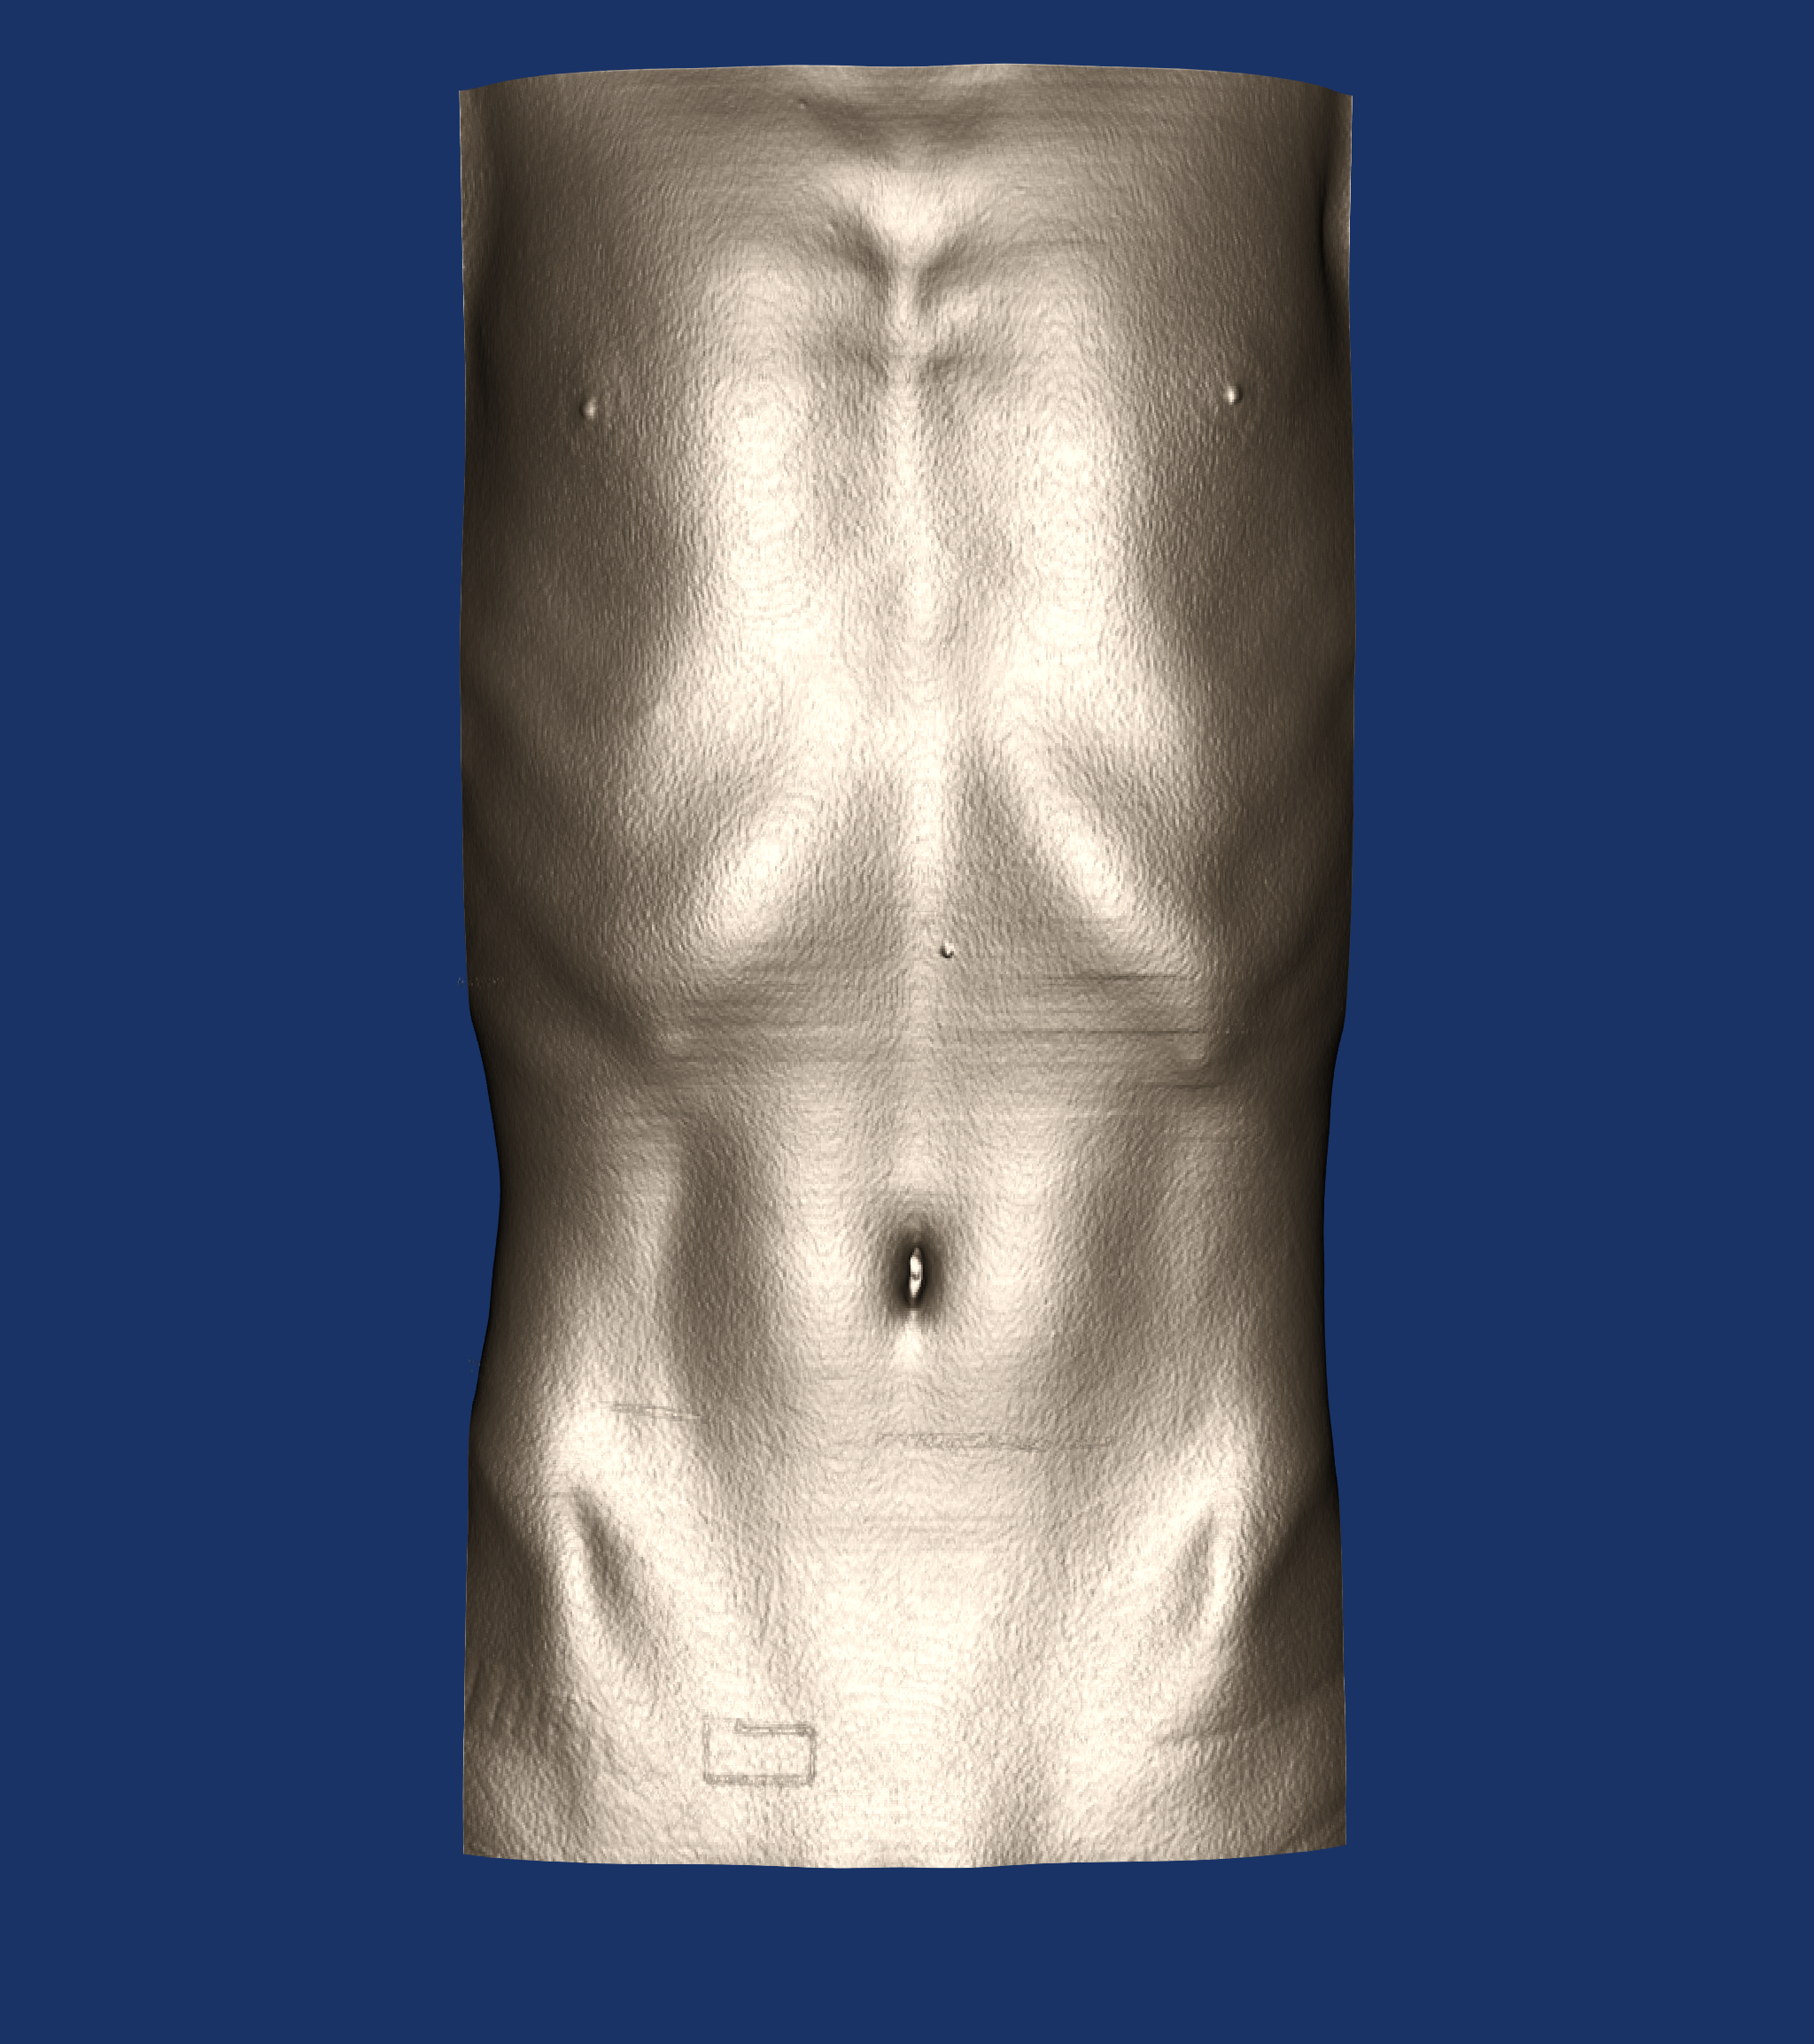
\includegraphics[width=1\linewidth]{TorsoNoGradient.png}
   \caption{}
   \label{fig:Ng2}
\end{subfigure}

\caption{Rendering with and without gradient opacity transfer function.}
\label{fig:gradient}
\end{figure*}

\subsubsection{Mobile Support}
The move to OpenGL 3 and higher enabled volume rendering to support mobile devices (iOS and Android devices) as OpenGL ES 3.0 and higher supports 3D textures. Support for multiple touch events such as using two fingers to translate, rotate, and zoom the camera was added to support interactive rendering on mobile devices. New texture formats are added with logistics to enable / disable them based on the platform.. With minor feature-set exceptions, the new volume mapper works on mobile devices enabling developers to build sophisticated applications for the scientific community.

\subsubsection{Volume Picking}
Picking is defined in this context as the effort of determining which on-screen object a user has clicked on,  this is one of the most basic operations to interact with a 3D scene. VTK legacy volume mappers support picking through an instance external to the mapper itself called vtkVolumePicker.  This class casts a ray into the volume and returns the point where the ray intersects an isosurface of a user specified opacity. This technique has certain limitations given that the picking class does not have enough information to correctly account for clipping, transfer functions and other parameters which define how the mapper renders internally, this reduces its reliability on the actual objects being picked.
The inherent flexibility of the glsl-based implementation of the new vtkGPURayCastMapper enables seamless integration with the vtkHardwareSelector's interface, which allows a consistent selection of objects in a scene regardless of whether it is geometric or volumetric data.  Providing picking support directly within the fragment shader of the volume mapper ensures high selection accuracy even in situations where a volume intermixes with geometry in seemingly cumbersome ways or advanced features like when clipping planes are enabled (what you see is what you pick).
Furthermore, this initial implementation supports a higher picking granularity than only the volume object itself (vtkProp).  Given the readily available picking styles supported by vtkHardwareSelector (e.g. vtkAreaPicker), it is possible to make a selection of a specific set of voxels.

\subsubsection{Lighting / Shading }
The old GPU ray cast mapper supported only one light (due to limitations in OpenGL at the time the class was written). The vtkFixedPointRayCastMapper supports multiple lights, but only with an approximate lighting model, since gradients are precomputed and quantized, and shading is performed for each potential gradient direction regardless of fragment location. The new vtkGPURayCastMapper accurately implemented the VTK lighting model to produce high quality images for publication. Up To six lights are supported (point, directional, and positional). The number of lights are limited to six mostly because of the performance reasons as the interactive performance goes down significantly with each light added to the scene. 

\subsubsection{Volume Texture Streaming}
An intrinsic limitation of volume rendering is that the texture to be rendered does not always fit into the graphics memory of a system. This becomes increasingly important to address now that the new mapper provides support for mobile architectures.
A relatively simple method when dealing with a large volume is the divide-and-conquer approach, which is sometimes referred to as bricking. The volume is split into several blocks in such a way that a single sub-block (brick) fits completely into GPU memory.  Each sub-block is stored in main memory and streamed into GPU memory for a rendering pass one at a time (in a back-to-front manner for correct composition). The sub-blocks are rendered using the standard shader programs and alpha-blended with each other by OpenGL.
Streaming the volume as separate texture bricks certainly imposes a performance trade-off but acts as a graphics memory expansion scheme for devices that would not be able to render a higher quality volume otherwise.